\documentclass[a4paper,10pt]{article}
\setlength{\parindent}{0cm}
\usepackage{amsmath, amssymb, amsthm, mathtools,pgfplots}
\usepackage{graphicx,caption}
\usepackage{verbatim}
\usepackage{venndiagram}
\usepackage[cm]{fullpage}
\usepackage{fancyhdr}
\usepackage{tikz}
\usepackage{listings}
\usepackage{color,enumerate,framed}
\usepackage{color,hyperref}
\definecolor{darkblue}{rgb}{0.0,0.0,0.5}
\hypersetup{colorlinks,breaklinks,
            linkcolor=darkblue,urlcolor=darkblue,
            anchorcolor=darkblue,citecolor=darkblue}
\usepackage[utf8]{inputenc}

% Default fixed font does not support bold face
\DeclareFixedFont{\ttb}{T1}{txtt}{bx}{n}{10} % for bold
\DeclareFixedFont{\ttm}{T1}{txtt}{m}{n}{10}  % for normal

% Custom colors
\usepackage{color}
\definecolor{deepblue}{rgb}{0,0,0.5}
\definecolor{deepred}{rgb}{0.6,0,0}
\definecolor{deepgreen}{rgb}{0,0.5,0}

\usepackage{listings}

% Python style for highlighting
\newcommand\pythonstyle{\lstset{
language=Python,
basicstyle=\ttm,
otherkeywords={self},             % Add keywords here
keywordstyle=\ttb\color{deepblue},
emph={MyClass,__init__},          % Custom highlighting
emphstyle=\ttb\color{deepred},    % Custom highlighting style
stringstyle=\color{deepgreen},
frame=tb,                         % Any extra options here
showstringspaces=false            % 
}}


% Python environment
\lstnewenvironment{python}[1][]
{
\pythonstyle
\lstset{#1}
}
{}

% Python for external files
\newcommand\pythonexternal[2][]{{
\pythonstyle
\lstinputlisting[#1]{#2}}}

% Python for inline
\newcommand\pythoninline[1]{{\pythonstyle\lstinline!#1!}}
%\usepackage{tgadventor}
%\usepackage[nohug]{diagrams}
\usepackage[T1]{fontenc}
%\usepackage{helvet}
%\renewcommand{\familydefault}{\sfdefault}
%\usepackage{parskip}
%\usepackage{picins} %for \parpic.
%\newtheorem*{notation}{Notation}
%\newtheorem{example}{Example}[section]
%\newtheorem*{problem}{Problem}
\theoremstyle{definition}
%\newtheorem{theorem}{Theorem}
%\newtheorem*{solution}{Solution}
%\newtheorem*{definition}{Definition}
%\newtheorem{lemma}[theorem]{Lemma}
%\newtheorem{corollary}[theorem]{Corollary}
%\newtheorem{proposition}[theorem]{Proposition}
%\newtheorem*{remark}{Remark}
%\setcounter{section}{1}

\newtheorem{thm}{Theorem}[section]
\newtheorem{lemma}[thm]{Lemma}
\newtheorem{prop}[thm]{Proposition}
\newtheorem{cor}[thm]{Corollary}
\newtheorem{defn}[thm]{Definition}
\newtheorem*{examp}{Example}
\newtheorem{conj}[thm]{Conjecture}
\newtheorem{rmk}[thm]{Remark}
\newtheorem*{nte}{Note}
\newtheorem*{notat}{Notation}

%\diagramstyle[labelstyle=\scriptstyle]

\lstset{frame=tb,
  language=Oz,
  aboveskip=3mm,
  belowskip=3mm,
  showstringspaces=false,
  columns=flexible,
  basicstyle={\small\ttfamily},
  breaklines=true,
  breakatwhitespace=true,
  tabsize=3
}


\pagestyle{fancy}




\fancyhead{}
\renewcommand{\headrulewidth}{0pt}

\lfoot{\color{black!60}{\sffamily Zhangsheng Lai}}
\cfoot{\color{black!60}{\sffamily Last modified: \today}}
\rfoot{\color{black!60}{\sffamily\thepage}}



\begin{document}
\flushright{Zhangsheng Lai\\1002554}
\section*{Statistics: Homework 2}

\begin{enumerate}
\item[6.3] Given $\hat{\theta} = 2\overline{X}_n$ and $X_1, \ldots, X_n \sim \text{Uniform}(0,\theta)$,
\begin{align*}
\text{\sffamily bias}(\hat{\theta}) & =\mathbb{E}(2\overline{X}_n)-\theta\\
& =2n^{-1}\mathbb{E}\left(\sum_{i=1}^{n}{X}_i\right)-\theta\\
& =2n^{-1}\sum_{i=1}^{n}\mathbb{E}\left({X}_i\right)-\theta\\
& =2n^{-1}\frac{n\theta}{2}-\theta=0\\
\text{\sffamily se}(\hat{\theta})^2 & = \mathbb{V}(2\overline{X}_n)\\
& = 4\mathbb{V}(\overline{X}_n)\\
&=4n^{-2}\mathbb{V}\left(\sum_{i=1}^{n}{X}_i\right)\\
&=4n^{-2}\sum_{i=1}^{n}\mathbb{V}\left({X}_i\right)\\
&=4n^{-2}\frac{n\theta^2}{12} = \frac{\theta^2}{3n}\\
\text{\sffamily MSE}(\hat{\theta}) &= \text{bias}(\hat{\theta})^2+\text{se}(\hat{\theta})^2 = \frac{\theta^2}{3n}
\end{align*}
\item[7.2] For $X_1, \ldots, X_n \sim \text{Bernoulli}(p)$ plug-in estimator for $p$ is 
\begin{align*}
\hat{p}=\frac{1}{n}\sum_{i=1}^{n}X_i
\end{align*}
and the estimated standard error is given by
\begin{align*}
\hat{\text{\sffamily se}}_p = \sqrt{\mathbb{V}(\hat{p})} = \sqrt{\frac{\hat{p}(1-\hat{p})}{n} }
\end{align*}
As the $X_i$'s are iid, by Central Limit Theorem, $\hat{p}$ is asymptotically normal with mean $p$ and variance $\hat{\text{\sffamily se}}_p^2$. Thus an approximate $90\%$ confidence interval for $p$ is $(\hat{p}-1.645\text{\sffamily se},\hat{p}+1.645\text{\sffamily se})$.

For $X_1, \ldots, X_n \sim \text{Bernoulli}(p)$ and $Y_1, \ldots, Y_n \sim \text{Bernoulli}(q)$ plug-in estimator for $p-q$ is 
\begin{align*}
\hat{p}-\hat{q}=\frac{1}{n}\sum_{i=1}^{n}X_i - \frac{1}{m}\sum_{i=1}^{m}Y_i
\end{align*}
with estimated standard error 
\begin{align*}
\hat{\text{\sffamily se}}_{p-q} = \sqrt{\mathbb{V}(\hat{p}-\hat{q})} = \sqrt{\mathbb{V}(\hat{p})+\mathbb{V}(\hat{q})}= \sqrt{\frac{\hat{p}(1-\hat{p})}{n}+\frac{\hat{q}(1-\hat{q})}{m} }
\end{align*}
Since the $Y_i$'s are iid, by Central Limit Theorem $\hat{q}$ is asymptotically normal with mean $q$ and variance $\hat{\text{\sffamily se}}_q^2$. The difference of two asymptotically normal random variables is asymptotically normal, thus $\hat{p-q}$ is asymptotically normal with mean $p-q$ and variance $\text{\sffamily se}_{p-q}^2$. An approximate $90\%$ confidence interval is 
\begin{align*}
%\text{\sffamily se}_{p-q}=
(\hat{p}-\hat{q}-1.645\text{\sffamily se}_{p-q},\hat{p}-\hat{q}+1.645\text{\sffamily se}_{p-q})
\end{align*}
\item[7.9] An estimate for $p_1-p_2$ is $0.9-0.85=0.05$ with standard error 
\begin{align*}
\sqrt{\frac{0.9(1-0.9)}{100}+\frac{0.85(1-0.85)}{100}}= 0.0466368953
\end{align*}
with $80\%$ and $90\%$ confidence intervals given by
\begin{align*}
80\%:\quad(\hat{p}-\hat{q}-1.282\text{\sffamily se}_{p-q},\hat{p}-\hat{q}+1.282\text{\sffamily se}_{p-q})&=(-0.0097885,0.1097885)\\
90\%:\quad(\hat{p}-\hat{q}-1.96\text{\sffamily se}_{p-q},\hat{p}-\hat{q}+1.96\text{\sffamily se}_{p-q})&=(-0.041408315,0.141408315)
\end{align*} 

\item[8.7]
\begin{enumerate}[(a)]
\item 
\begin{align*}
\mathbb{P}(\hat{\theta}\leq k) &= \mathbb{P}(\max\{X_1,\ldots,X_n\}\leq k)\\
&= \prod_{i=1}^{n}\mathbb{P}(X_i\leq k)\\
&=\left(\frac{k}{\theta}\right)^n
\end{align*}
\begin{figure}[h]
\centering
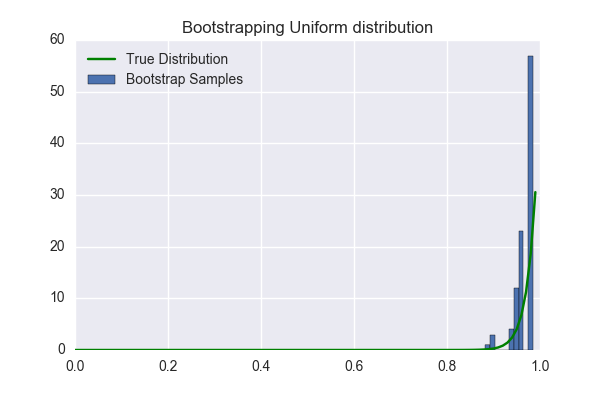
\includegraphics[scale=1]{bootstrap1.png}
\caption{Comparison of the true distribution $\hat{\theta}$ to histrograms from bootstrap}
\end{figure}

Code for the plot:
\begin{python}
import numpy as np
import matplotlib.pyplot as plt
def sample(theta, n):
    """
    Draws n samples from uniform distribution in the interval (0, theta).
    """
    return np.random.uniform(0, theta, n)

def bootstrap(sample, B):
    """
    Performs bootstrapping B times from the given sample.
    """
    n = sample.shape[0]
    bootstrap = np.zeros((B,50))
    for i in range(B):
        bootstrap[i,:] = np.random.choice(sample, 50)
    return bootstrap
def maxestimator(bootstrap):
    """
    Returns the maximum value from each bootstrap sample.
    """	
    return np.max(bootstrap, axis = 1)
def plotcdf(theta, n):
    """
    Plots the true distribution of the X_max
    """
    x = np.arange(0, theta, 0.01)
    f = lambda x: n*(x/theta) ** (n-1) 
    y = f(x)
    plt.plot(x, y, 'g', label = 'True Distribution')
def finalplot(theta, n, B):
    """
    Plots both the simulations and the true distribution for comparison.
    """	
    samples = sample(theta, n)
    bootstraps = bootstrap(samples, B)
    max_samples = maxestimator(bootstraps)
    plt.hist(max_samples, label = 'Bootstrap Samples')
    plotcdf(1, 50)
    plt.legend(loc='best')
    plt.title('Bootstrapping Uniform distribution')
finalplot(1, 50, 100)                    
\end{python}
\item Let $\hat{\theta} = X_{max} = \max\{X_1, \ldots, X_n\}$. Then
\begin{align*}
\mathbb{P}(\hat{\theta}^\ast = \hat{\theta})&=1-\mathbb{P}(\hat{\theta}^\ast \neq \hat{\theta})\\
&=1 - \left(1-\frac{1}{n}\right)^n
\end{align*}
The second equality holds as $\mathbb{P}(\hat{\theta}^\ast \neq \hat{\theta})$ denotes the probability that any random sampling with replacement of the $n$ samples drawn has probability of $1-1/n$ not being $x_{max}$ (which is fixed since a random sample of $n$ has been drawn). As each sampling process is iid due to replacement, probability of them all not being $x_{max}$ is $(1-1/n)^n$. Thus we have $\mathbb{P}(\hat{\theta}^\ast = \hat{\theta}) \to 0$ as $n \to \infty$ and $\mathbb{P}(\hat{\theta}^\ast = \hat{\theta}) = .632$ for $n=50$.
\end{enumerate}
\item[9.2]
\begin{enumerate}[(a)]
\item For $X_1,\ldots, X_n \sim \text{Uniform}(a,b)$
\begin{align*}
\hat{\mu}=\overline{X}_n=\frac{1}{n}\sum_{i=1}^{n}X_i&=\frac{\hat{b}+\hat{a}}{2}\\
\hat{\sigma}^2=\frac{1}{n}\sum_{i=1}^{n}(\overline{X}_n-X_i)^2&=\frac{(\hat{b}-\hat{a})^2}{12}
\end{align*}
thus
\begin{align*}
(\hat{b}-\hat{a})+(\hat{b}+\hat{a}) &= +\sqrt{12\hat{\sigma}^2}+2\hat{\mu}\\
\hat{b} &= \frac{1}{2}\left(\sqrt{12\hat{\sigma}^2}+2\hat{\mu}\right)\\
\hat{a} &=2\hat{\mu}-\hat{b }
\end{align*}
the positive root is taken as $b-a>0$.
\item Let $X_1,\ldots, X_n \sim \text{Uniform}(a,b)$, with $X_{max}=\max \{X_1,\ldots, X_n\}$. If $b < X_{max}$, then $f(X_j;a,b)=0$ for some $j$. Thus if $b \geq X_{max}$, then $f(X_i;a,b)=1/b-a$ for all $i$. In a similar fashion, letting $X_{min} = \{X_1,\ldots, X_n\}$, if $X_{min}<a$ we also have $f(X_j;a,b)=0$ for some $j$ and $f(X_i;a,b)=1/b-a$ for all $i$ if $X_{min} \geq a$. Therefore,
\begin{align*}
\mathcal{L}_n(a,b):=\begin{cases}
0, & X_{min} < a \text{ or }X_{max} >  b \\
\left(\frac{1}{b-a}\right)^n, & \text{ otherwise }%X_{max} \leq b \text{ and } X_{min} \geq a
\end{cases}
\end{align*}
$\mathcal{L}(a,b)$ strictly decreasing over $(-\infty,X_{min}]$ and $[X_{max},\infty)$, thus the maximum likelihood estimators $\hat{a}=X_{min}$ and $\hat{b}=X_{max}$.

\item Let $\tau = \int x \,dF(x)$ be given, then from (b) we know that {\sffamily MLE}'s $\hat{a}$ and $\hat{b}$ are given by $X_{min}$ and $X_{max}$ respectively. Then the {\sffamily MLE} of $\tau$ follows from {\sffamily MLE}'s $\hat{a}$ and $\hat{b}$. Thus {\sffamily MLE} of $\tau$ is $(X_{min} + X_{max})/2$. 
\item By simulation, the {\sffamily MSE} of $\hat{\tau} \approx 0.015$ by using the Python code below:
\begin{python}
import numpy as np
n = 500000
mle_tau = np.zeros((n,1))
for i in np.arange(n):
    s = np.random.uniform(1, 3, 10)
    s_max = np.max(s)
    s_min = np.min(s)
    mle_tau[i] = 0.5 * (s_max + s_min)
(1/n) * np.sum((mle_tau - 2) **2)    
\end{python}

Analytically, for the {\sffamily MSE} of the  nonparametric plugin estimator $\tilde{\tau}$ we have

\begin{align*}
\mathbb{E}(\hat{\theta}-\theta)^2&=\mathbb{E}(\hat{\theta}^2-2\hat{\theta}\theta+\theta^2)\\
&=\mathbb{E}(\hat{\theta}^2)-2\theta\mathbb{E}(\hat{\theta})+\mathbb{E}(\theta^2)\\
&=\mathbb{E}(\hat{\theta}^2)-2\theta\mathbb{E}(\hat{\theta})+\mathbb{E}(\theta^2)\\
&=\mathbb{E}(\hat{\theta}^2)-4
\end{align*}
\begin{align*}
\mathbb{E}(\hat{\theta})^2&=n^{-2}\left[\mathbb{E}\left(\sum_{i=1}^{n}X_i^2\right)+2\mathbb{E}\left(\sum_{i\neq j}X_iX_j\right)\right]\\
&=n^{-2}\left[n\mathbb{E}\left(X^2\right)+n(n-1)\mathbb{E}\left(X_iX_j\right)\right]\\
&=n^{-2}\left[n\mathbb{E}\left(X^2\right)+n(n-1)\mathbb{E}\left(X\right)^2\right]\\
&=121/30
\end{align*}
using the substitution $\mathbb{E}(X^2) = 2 $, $\mathbb{E}(X) = 13/2$ and $n=10$. The expectations are computed with $a=1, b=2$. Thus we have {\sffamily MSE} to be $1/30$.
\end{enumerate}
\item[9.6] 
\begin{enumerate}[(a)]
\item The log-likelihood function is given to be
\begin{align*}
\ell_n(\theta)&=n\log\frac{1}{\sqrt{2\pi}}-\sum_{i=1}^{n}\frac{(X_i-\theta)^2}{2}\\
&=n\log\frac{1}{\sqrt{2\pi}}-\frac{n}{2}S^2-\frac{n}{2}(\overline{X}_n-\theta)^2\\
\text{with } \frac{\partial \ell_n}{\partial \theta}&=n(\overline{X}_n-\theta)
\end{align*}
where $\overline{X}_n = n^{-1}\sum_{i=1}^{n} X_i$. Thus the maximum of the log-likelihood function is when $\theta = \overline{X}_n$. Now, $X_1 \sim N(\overline{X}_n,1)$ and so the maximum likelihood of $\psi$ is given by:
\begin{align*}
%X_1 >0 &\Leftrightarrow n\theta - \sum_{i=2}^{n}X_i > 0\Leftrightarrow \theta > n^{-1}\sum_{i=2}^{n}X_i \\
\hat{\psi} = \mathbb{P}(X_1 >0) &= \mathbb{P}\left(X_1 -\overline{X}_n > -\overline{X}_n\right)\\
&= \mathbb{P}\left( Z> -\overline{X}_n\right)\\
\end{align*}
where the $Z$ refers to the standard normal distribution.
%\item We observe that with $\psi = \mathbb{P}(Y_1=1)$ the $Y_i$'s have a Bernoulli distribution with parameter $\psi$. Thus the variance of $\psi$ is $\psi(1-\psi)$
\item
By Central Limit Theorem, we know that 
\begin{align*}
\sqrt{n}(\overline{X}_n-\theta) \leadsto N(\theta, 1)
\end{align*}
defining $g(\theta) = \psi = \mathbb{P}(Y_1=1) = \mathbb{P}(X_1>0)$ we have
\begin{align*}
\frac{g(\overline{X}_n)-g(\theta)}{|g'(\overline{X}_n)|\hat{\text{\sffamily se}}(\overline{X}_n)}\leadsto N(0,1)
\end{align*} 
thus the $\hat{\text{\sffamily se}}$ for the confidence interval is $|g'(\overline{X}_n)|\hat{\text{\sffamily se}} = \frac{1}{\sqrt{2n\pi}}\exp (-1/2(\overline{X}_n)^2)$. Thus the confidence interval is given by:
\begin{align*}
\mathbb{P}\left( Z> -\overline{X}_n\right) \pm 1.96\frac{1}{\sqrt{2n\pi}}\exp (-1/2(\overline{X}_n)^2)
\end{align*}
%\item The distribution of $\hat{\psi}$ is normally distributed with $\hat{\text{\sffamily se}} = \sqrt{1/I_n(\hat{\theta})}$
%\begin{align*}
%I_n(\theta) &= nI(\theta)\\
%&= nI(\theta)\\
%\end{align*}
%Since $f(X;\theta) = 1/\sqrt{2\pi}\exp(-1/2(X-\theta)^2)$, we have the score function $s(X;\theta) = X - \theta$ and $s'(X;\theta) = 1$. Thus $I(\theta) = -\mathbb{E}_\theta(s'(X;\theta))=-1$. Hence $\hat{\text{\sffamily se}} = 1/\sqrt{n}$ which gives us a 95 percent confidence interval of $\mathbb{P}\left( Z> -\overline{X}_n\right) \pm 1.96/\sqrt{n}$
\item Let $\tilde{\psi} = (1/n)\sum_iY_i$, to show $\tilde{\psi}$ is consistent, we need to show that $\mathbb{P}(|\tilde{\psi} - \psi|>\epsilon) \to 0$ as $n \to \infty$. We also observe that $Y\sim \text{Bernoulli}(p)$ where $p = \mathbb{P}(X>0)$
\begin{align*}
\mathbb{P}(|\tilde{\psi} - \psi|>\epsilon) &= \mathbb{P}(|(1/n)\sum_iY_i - \mathbb{P}(Y_1=1)|>\epsilon)\\
&=\mathbb{P}\left(\left|\sum_iY_i - n\mathbb{P}(Y_1=1)\right|^2>(\epsilon n)^2\right)\\
&\leq \mathbb{E}\left(\left[\sum_iY_i - n\mathbb{P}(Y_1=1)\right]^2\right)/(\epsilon n)^2\quad \text{by Markov's inequality}\\
&=\frac{n\mathbb{E}(Y)-n\mathbb{E}(Y)^2+\left(n\mathbb{E}(Y)-n\mathbb{P}(Y_1=1)\right)^2}{\epsilon^2n^2}\\
&\to \frac{(\mathbb{E}(Y)-\mathbb{P}(Y_1=1))^2}{\epsilon^2}=0 \text{ as } n \to \infty
\end{align*}
\item We are given $\tilde{\psi} = \overline{Y}_n = n^{-1}\sum_{i=1}^{n}Y_i$ with $Y \sim \text{Bernoulli}(p)$, $p = \mathbb{P}(Z>-\theta)$. Thus by Central Limit Theorem,
\begin{align*}
\frac{\overline{Y}_n-\mathbb{E}(Y)}{\sqrt{\mathbb{V}(Y)/n}} \leadsto N(0,1)
\end{align*}
thus $\overline{Y}_n$ is normally distributed with mean $p$ and variance $p(1-p)/n$. Next we consider the {\sffamily MLE}, $\hat{\psi}$. We know from (a) that $\psi(\theta) = \mathbb{P}(Z > -\theta)$ with $X \sim N(\theta, 1)$ and $\hat{\psi} = \psi(\overline{X}_n)$. By Central Limit Theorem,
\begin{align*}
\frac{\overline{X}_n - \theta}{1/\sqrt{n}} \leadsto N(0,1)
\end{align*}
and $\hat{\psi}$ is differentiable since it is a complementary cumulative distribution function and its derivative is strictly greater than 0. Therefore,
\begin{align*}
\frac{\psi(\overline{X}_n) - \psi(\theta)}{|\psi'(\overline{X}_n)|} \leadsto N(0, 1)
\end{align*}
evaluating $\psi'(\overline{X}_n)$, we have the probability distribution function evaluated at $\overline{X}_n$ which is 
\begin{align*}
f_X(\overline{X}_n)=\frac{1}{\sqrt{2\pi}} \exp( -1/2(\overline{X}_n))
\end{align*}
Letting $f_Z(z)$ and $\overline{F}_Z(z)$ denote the pdf and complementary cdf of a normal distribution with mean $0$ and variance 1, the asymptotic relative efficiency of $\tilde{\psi}$ to $\hat{\psi}$ is 
\begin{align*}
\text{\sffamily ARE}(\tilde{\psi}, \hat{\psi}) = \frac{\overline{F}_Z(-\theta)(1-\overline{F}_Z(-\theta))}{\left(f_Z(\overline{X}_n)\right)^2}
\end{align*}
%Using the delta method, we have the standard error of the {\sffamily MLE} denoted $\hat{\text{\sffamily se}}$....
%The standard error of $\tilde{\psi}$ denoted by $\tilde{\text{\sffamily se}}$
\item If the data is not normal, unless it is a constant distribution, it will be consistent due to Central Limit Theorem. Let $X_i =-1$ for all $i$, i.e. no matter how many times you sample you only get -1. Thus 
\begin{align*}
\hat{\psi}= \mathbb{P}(Z > -1) \neq 0 = \mathbb{P}(Y_1=1) = \psi
\end{align*}
\end{enumerate}
\end{enumerate}

\end{document}